





\begin{figure}
\begin{center}
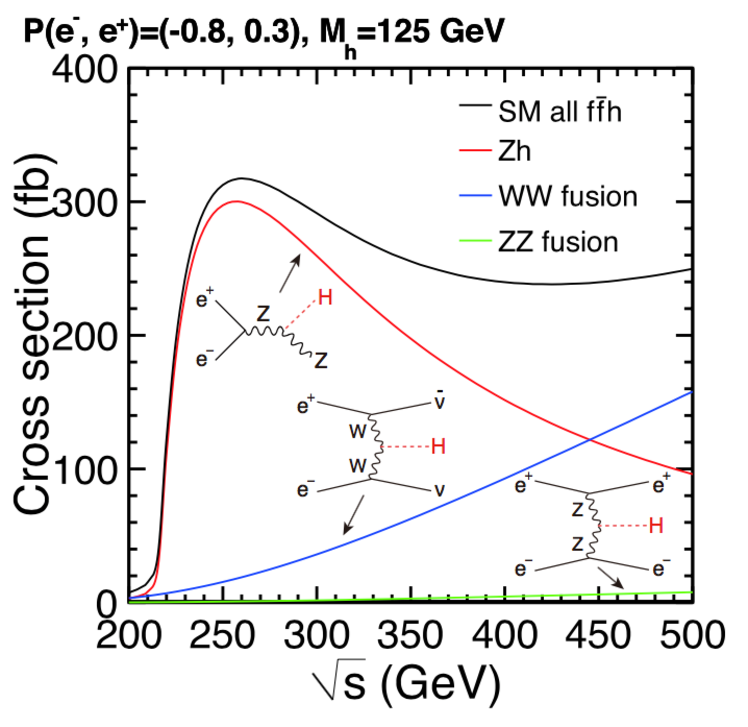
\includegraphics[width=0.85\hsize]{chapters/figures/xsec_h_ILC_left.pdf}
\end{center}
\caption{Cross sections for the three major Higgs production processes
  as a function of 
center of mass energy, 
from~\cite{Baer:2013cma}.}
\label{fig:HiggsProdILC}
\end{figure}


The physics case for the precision study for the Higgs
boson
presented  in Section~\ref{sec:physics}
will be realized through the measurement of  total cross sections and 
$\sigma\cdot BR$  values for the various final-states.  The major
Higgs production cross sections at the ILC are shown in
Fig.~\ref{fig:HiggsProdILC} as a function of centre of mass energy for
the optimal choice of  ILC beam polarization.    In
Tab.~\ref{tab:higgserrors},  we present our estimates for the
statistical errors that will be obtained for the total cross section for $\ee\to ZH$ and for
the $\sigma\cdot BR$s for  this process and the $WW$ fusion process, 
for a reference luminosity sample of 
250~\ifb\ and for three different ILC energies.  These estimates are
based on full-simulation analyses using the tools presented in
Sec.~\ref{sec:software}.     The purpose of this
section is explain how these numbers are obtained, what the factors
are  that limit them, and how these limitations might be relaxed.


\begin{table}[htb]
\begin{center}
%\begin{tabular} {lcccccc}
\begin{tabular} {lcccccc}
\multicolumn{7}{l} {-80\% $e^-$, +30\% $e^+$ polarization:} \\  \hline
% & 250 GeV   &  & 350 GeV & & 500 GeV  &  \\
 & \multicolumn{2}{c}{250 GeV} & \multicolumn{2}{c}{350 GeV}  & \multicolumn{2}{c}{500 GeV} \\
 &  $Zh$ & $ \nu\bar\nu h$  & $ Zh$ & $\nu\bar\nu h$ & $Zh$ & $ \nu\bar\nu h$\\ 
\hline
$\sigma$  &    2.0     &    &1.8  &  &  4.2   &     \\  \hline
$h\to invis.$ &  0.86   &  &1.4 &   &   3.4 &     \\
\hline
$h\to b\bar b$  &   1.3 &  8.1 & 1.5  &  1.8  & 2.5  &  0.93  \\ 
$h\to c\bar c$ &  8.3 &   &11 & 19  &   18 & 8.8 \\ 
$h\to gg$ &  7.0 &  &8.4  & 7.7 & 15  &  5.8\\
$h\to WW$  &  4.6 &   &5.6$^*$ & 5.7$^*$ &  7.7   &  3.4\\
$h\to \tau\tau$  & 3.2 &   &4.0$^*$ & 16$^*$ &  6.1  &  9.8\\
$h\to ZZ$ & 18 &   & 25$^*$ & 20$^*$ & 35$^*$  & 12$^*$    \\ 
$h\to \gamma\gamma$  & 34$^*$ &   &39$^*$ &  45$^*$ &  47 &  27 \\ 
$h\to \mu\mu$ & 72 &   &87$^*$&  160$^*$ &  120 &  100 \\
\hline\hline
$a$  &  7.6   &     &2.7$^*$ &   &  4.0   &  \\
$b$ &  2.7  &    & 0.69$^*$ &    & 0.70   &   \\
$\rho(a,b)$  &  -99.17 &   & -95.6$^*$ &  & -84.8 &   \\
\end{tabular}
\caption{Projected statistical errors, in \%, for Higgs boson 
measurements. The errors are 
quoted for luminosity samples of 250~fb$^{-1}$
  for $\ee$ beams with -80\% electron polarization and +30\% positron
  polarization. 
  Except for the first and last segments of  each set, these are measurments
  of  $\sigma \cdot BR$, relative to the Standard Model
  expectation.
The top lines gives the error for the total cross section relative to
the Standard Model and  the 95\% confidence upper limit on the branching ratio for
Higgs to invisible decays.  The bottom lines in each half give the
expected errors on the $a$ and $b$ parameters and their correlation
(all in \%)  for $\ee\to Zh$ (see
\leqn{eqn:CPHZZ}.    All error estimates in this table are
based on full simulation, and the entries marked with a $^*$ are 
extrapolated from full simulation results. }  
\label{tab:higgserrors}
\end{center}
\end{table}

%\begin{table}
%\begin{center}
%\begin{tabular} {lcccccc}
% & 250 GeV   &  & 350 GeV & & 500 GeV  &  \\
% &  $ W^+ W^-$  &  &  $ W^+ W^-$  &  &  $ W^+ W^-$  & \\
% \hline
%$g_{1Z}$ & 0 .062$^*$&   &0.033$^*$ &  &0.025  &  \\
%$\kappa_A $ & 0.096$^*$ &   & 0.049$^*$  &   & 0.034 &  \\
%$\lambda_A$ &   0.077$^*$ &   &0.047$^*$  &  &0.037  &  \\
%$\rho(g_{1Z},\kappa_A)$ & 63.4$^*$ &   &63.4$^*$  &  & 63.4 &  \\
%$\rho(g_{1Z},\lambda_A)$ &  47.7$^*$ &   & 47.7$^*$  &  &47.7  &  \\
%$\rho(\kappa_A,\lambda_A)$ & 35.4$^*$  &   & 35.4$^*$  &  & 35.4  &  
%\end{tabular}
%\caption{Projected statistical errors, in \%, for $\ee\to W^+W^-$
%measurements input to our fits. The errors are 
%quoted for luminosity samples of 500~fb$^{-1}$   divided equally
%between beams with 
 %-80\% electron polarization and +30\% positron
 % polarization and  brams with  +80\% electron polarization and -30\% positron
  %polarization. The last three lines give the correlation
  %coefficients, also in \%.  All error estimates in this table are
%based on full simulation, and the entries marked with a $^*$ are 
%extrapolated from full simulation results. }
%\label{tab:WWerrors}
%\end{center}
%\end{table}


\begin{table}
\begin{center}
\begin{tabular} {lcccccc}
%measurement  & efficieny & S/B pre. & S/B final. \\
%\hline
%$\sigma_{Zh}$ in $\mu^+\mu^-h$  & 88\% & 1/43 & 1/1.3 \\
%$BR(h\to b\bar{b})$ in $q\bar{q}h$ & 33\% & 1/340 & 1/0.89 \\
%$BR(h\to\tau\tau)$ in $q\bar{q}h$ & 37\% & 1/52 & 1/0.44 \\
%$BR(h\to WW)$ in $\nu\bar{\nu}h$ & 20\% & 1/87 & 1/1.6 \\
measurement  & efficieny &  S/B final. \\
\hline
$\sigma_{Zh}$ in $\mu^+\mu^-h$  & 88\% & 1/1.3 \\
$BR(h\to b\bar{b})$ in $q\bar{q}h$ & 33\% & 1/0.89 \\
$BR(h\to\tau\tau)$ in $q\bar{q}h$ & 37\% &  1/0.44 \\
$BR(h\to WW)$ in $\nu\bar{\nu}h$ & 20\% &  1/1.6
\end{tabular}
\caption{Typical signal efficiencies (second column) and signal over background ratio (S/B) 
after the final cuts (third column) for some of the 
representative Higgs measurements (first column) at the ILC.}
\label{tab:ILCEffSB}
\end{center}
\end{table}


\begin{figure}
\begin{tabular}[c]{c}
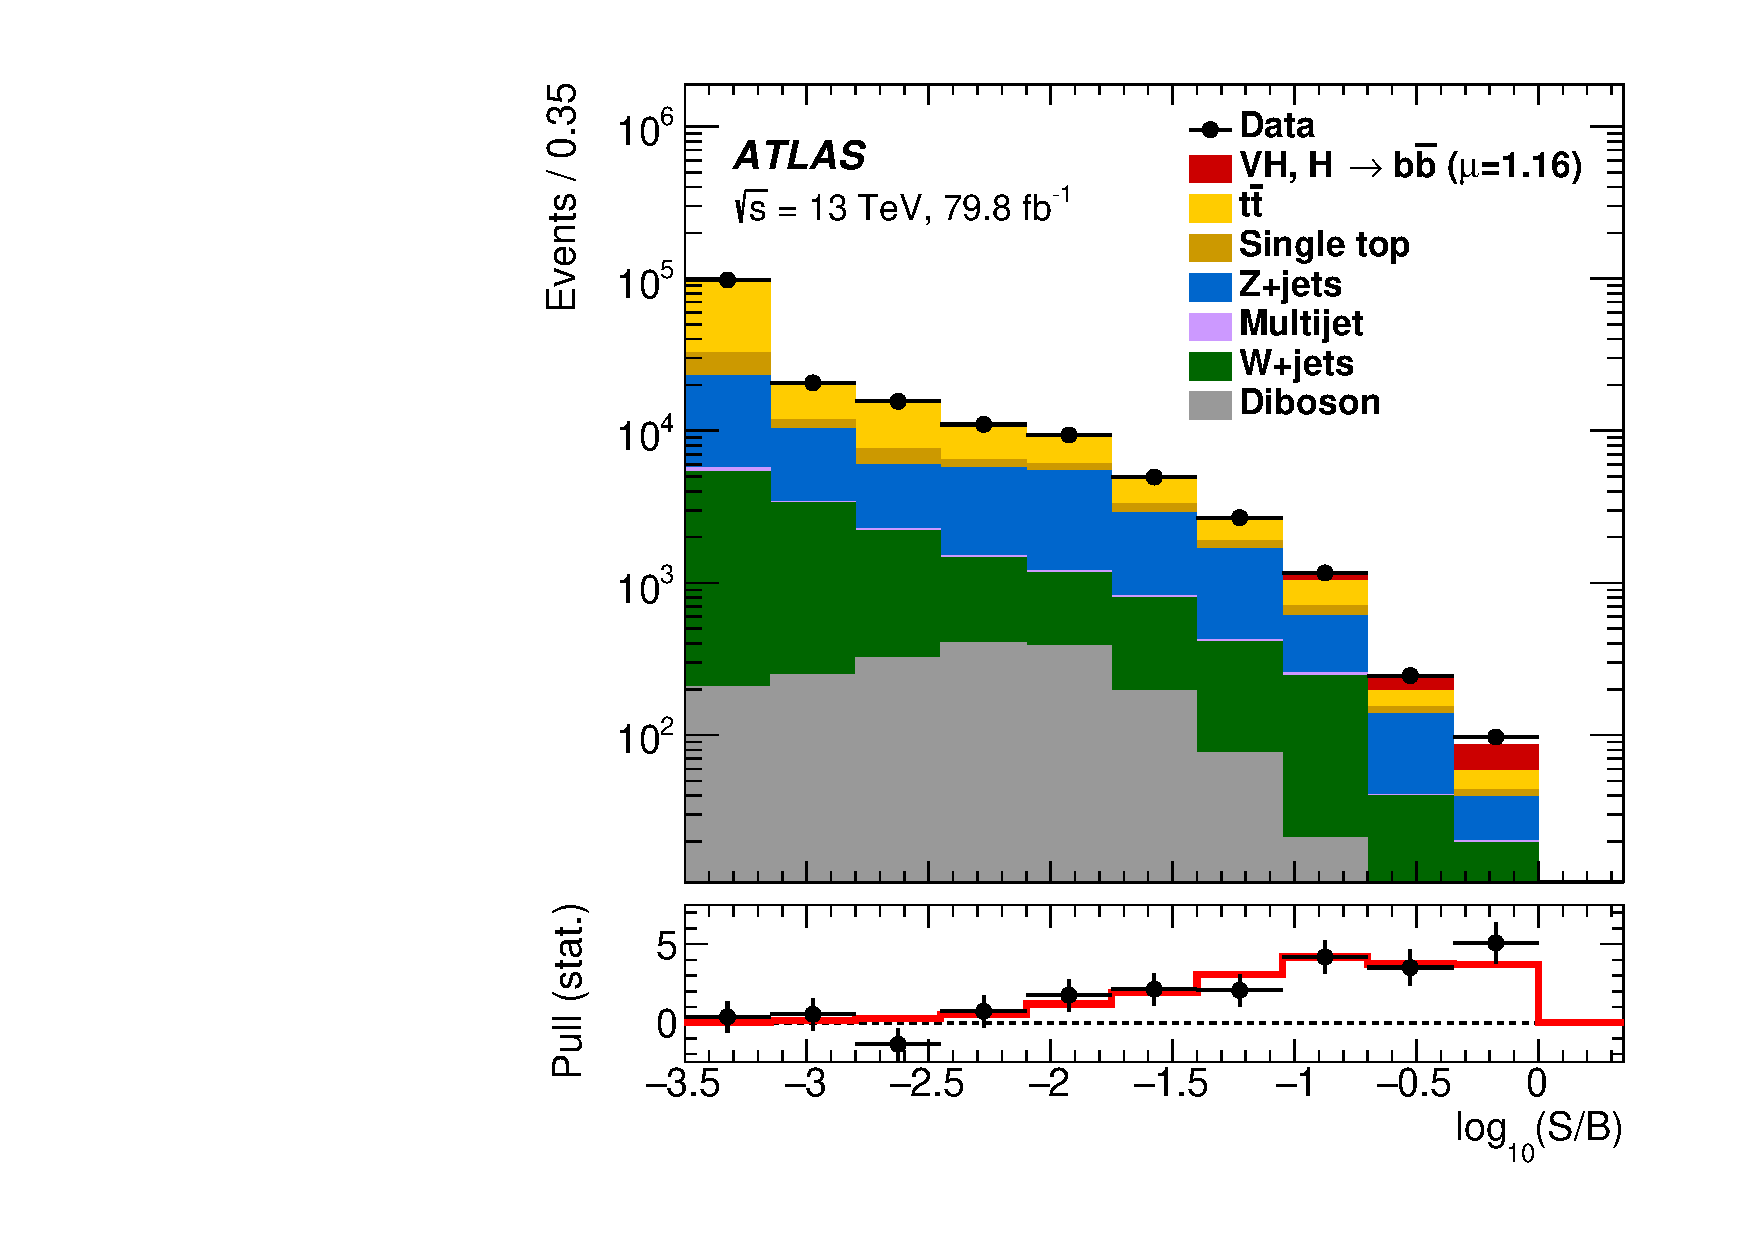
\includegraphics[width=0.85\hsize]{chapters/figures/ATLAS_VH_bb.pdf} \\
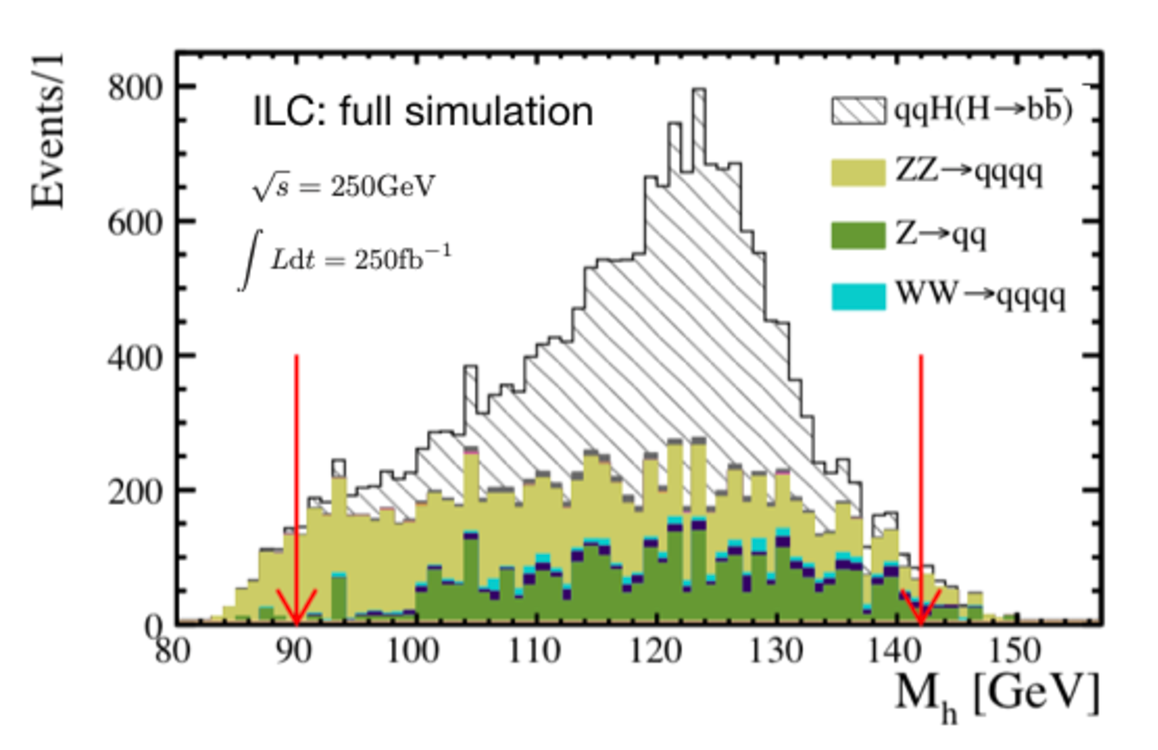
\includegraphics[width=0.85\hsize]{chapters/figures/qqH_bb250_ILC.pdf}
\end{tabular}
  \caption{Upper: signal $H\to b\bar{b}$ and background events in different categories of S/B
  measured by ATLAS~\cite{Aaboud:2018zhk,Sirunyan:2018kst} using LHC Run 2 data; lower: signal $h\to b\bar{b}$ 
  and background events in the $b\bar{b}$ mass spectrum expected from the 
  ILC full simulation~\cite{Ogawa:2018}.}
  \label{fig:LHCILCHbb}
\end{figure}




We begin from the observation that 
precision Higgs measurements will be much easier to obtain 
at a lepton collider than  at a hadron collider.
Table~\ref{tab:ILCEffSB} gives the typical signal efficiencies for ILC
analyses and the corresponding signal to
background ratios (S/B) after final cuts. The difference with
LHC can be clearly seen using the example of $H\to b\bar{b}$ measurements.
The decay of $H\to b\bar{b}$
has been discovered by ATLAS and
CMS~\cite{Aaboud:2018zhk,Sirunyan:2018kst} 
with a significance of 5.4$\sigma$, 5.5$\sigma$, respectively, 
after producting  about  4 million Higgs events per experiment.  At
the ILC,  with only 400 Higgs events which will be produced with an
 integrated luminosity of 1.3 fb$^{-1}$ (corresponding to 2 days of
 running time),
the decay of $H\to b\bar{b}$ will be 
measured with a similar significance, around 5.2$\sigma$ according to the full 
simulation result~\cite{Ogawa:2018}.  The S/B ratios for these
analyses are illustrated in  Fig.~\ref{fig:LHCILCHbb}. Clearly, if one
wishes to measure the rate for $h\to b\bar b$,
there are strong advantages in starting from a situation in which the
signal stands well above any background process that would need to be
controlled.   The challenge of physics at a linear collider is to make use of this
advantage in the most optimal way and realize the potential to achieve 
very high precision.


A full simulation analysis contains two components.  The first is the 
detector simulation.  This provides  the 
realistic interactions between each final state particle and 
any part of the detector that the particle passes through, including new creation of
particles during the interaction; concrete algorithms for tracking,
particle flow analysis, vertex reconstruction and particle identification; 
the resulting performance of the various detector resolutions for track momentum, jet energy,
and impact parameters; and the  efficiencies for tracking, flavor tagging, 
and isolated lepton finding.  These aspects have already been
described in Section~\ref{sec:software}. The second component
 is the event seletion, that is, the algorithms
for discriminating
between signal and background events. That will be our main concern in
the discussion of this section.

First, however, we would like to emphasize to the reader a number
of effects that are included in the detector modelling and event
generation, and that must be included for a solid estimate of
detection efficiencies and signal-background discrimination:
\begin{itemize}
\item {\it beamstrahlung and ISR}
are implemented in the event generators for both signal and background processes.
These effects are important for estimation of 
signal and background contributions in the analyses that make use of the 
nominal value of the centre-of-mass energy. A representative example is seen in
Section~\ref{sec:higgs:sigmazh}, Fig.~\ref{fig:RecoilMassLep250}, for
the determination of the Higgs boson mass from $Z$ recoil. 
Both beamstrahlung and ISR effects will drag signal events
from the more sensitive peak region to the less sensitive tail region,
and at the same time will induce more background contribution in the signal region.
\item {\it overlay of beam background events} is implemented in every signal 
and background event sample.  This will affects the performance of 
reconstructed variables related to jets and  hence degrades the signal and background
discrimination. There is a method to partially remove the effect of
this events which will 
be introduced in next section. 
\item {\it full standard model background} is checked in all of  the
  analyses to be described,
in order not to miss any significant contribution. For example,  2-fermion 
events developed with a parton shower can   become background for the  4-fermion signal.
Another example is the background contribution to  Higgs observables
that 
comes from tail of the Breit-Wigner structure of a $Z$ boson in
$\ee\to ZZ$.   It is not correct either to neglecting the 
$Z$ natural width nor to ignore the  similar diagram with the $\gamma$ propagator.
\item {\it explicit jet clustering and jet paring} algorithms are used
  in all analyses.   These often become the 
limiting factors the analyses with 4 or more jets  in the final state.
The confusion between two color singlets, for instance $Z$ and $h$ in $\ee\to Zh\to 4 jets$,
could produce a much wider spread of the reconstructed dijet invariant mass
than that due to  the pure detector resolution. Hence,  simply
smearing the  dijet mass variable 
at the parton level according to the detector resolution is often too optimistic. 
\item {\it control of systematics} is taken into account in the design of every
selection cut.
\end{itemize}



This section is organized as follows. In
Sec.~\ref{subsec:higgs_common},  we will introduce  the common
procedures for event selections will be
introduced. Sec.~\ref{subsec:higgs_ana} will discuss the 
analyses for the main Higgs observable. The analysis strategies and 
selection cuts in some representative channels will be  discussed in great detail. 
Section~\ref{subsec:higgs_improve}  presents some estimates for
improvement of the key algorithms in the future.
Section~~\ref{subsec:higgsself}  gives a dedicated discussion of the 
 measurement of Higgs self-coupling.